\chapter{Impostazione del problema di ricerca}
\label{chap:impost_prob_ricerca}

Il nostro lavoro si è concentrato principalmente allo studio di situazioni reali particolari, nelle quali si presentano delle problematiche relative ai canali di comunicazione. Più in particolare ci siamo concentrati a studiare quelle situazioni in cui i normali canali di comunicazione telefonica di rete fissa e mobile, internet compreso, non sono disponibili. Scenari di questo tipo sono, ad esempio, situazioni causate da intensi fenomeni di tipo meteorologico come forti nubifragi, temporali, grosse nevicate ed altri ancora. Nelle situazioni appena elencate, è facile che tali eventi atmosferici possano intaccare l'infrastruttura di telecomunicazione, rendendola non utilizzabile e causando non pochi problemi. Sappiamo bene che in casi di questo tipo, si rischia di rimanere senza comunicazioni e altri servizi anche per più di un giorno, a causa delle difficoltà nelle riparazioni dovute magari a ingenti danni alle infrastrutture. Il nostro studio si è concentrato nel cercare di analizzare questo tipo di scenari e provare a progettare una soluzione in grado di offrire un primo metodo per la diffusione di informazioni tra le persone su larga scala. Il nostro lavoro quindi, è mirato alla ricerca un possibile modo di diffondere messaggi e informazioni tra la popolazione, in situazioni dove le principali reti di comunicazione non sono disponibili. A questo punto, ci siamo quindi concentrati su ciò che rimane disponibile in queste situazioni e su cosa si possa sfruttare per costruire un sistema di comunicazione di emergenza. La nostra attenzione si è quindi spostata su l'analisi dell'ambiente e su tutto ciò rimane utilizzabile e fruibile anche durante una situazione di emergenza. Partendo dal fatto che il sistema avrebbe dovuto utilizzare una piattaforma tecnologica e che per essere un sistema di diffusione di massa, questa piattaforma dovrebbe essere un qualcosa di ampiamente diffuso, conosciuto e facilmente utilizzabile dalle persone. Da un indagine ISTAT \cite{istat2014} del 18 Dicembre 2014, le percentuali sulla presenza della tecnologia all'interno delle famiglie italiane sono tutte in crescita, come la presenza di una connessione a Internet salita 64\% o di una connessione a banda larga salita a quasi il 63\%, ma dato ancor più significativo è quello dei telefoni cellulari, che sono presenti in più del 93\% delle famiglie italiane. L'uso di Internet tramite smartphone è cresciuto dal 20.8\% al 28\% e ciò sta a indicare un rinnovamento anche nei dispositivi stessi; le persone acquistano dispositivi più recenti che permettano loro di navigare più facilmente su Internet. Sempre dall'analisi ISTAT è emerso che il 22.4\% delle persone che navigano su Internet dai 14 anni in su lo ha fatto tramite un computer, mentre il 35.4\% degli utenti tramite cellulare o smartphone e solo il 6\% da altri dispositivi mobili. L'utilizzo dello smartphone è la tipologia di dispositivi più utilizzata per l'accesso a Internet. Da questa indagine abbiamo pensato che uno dei dispositivi di estrema diffusione e di maggior utilizzo dalle persone, anche per l'accesso a Internet, è il telefono cellulare e più nello specifico, la categoria degli smartphone. A questo punto ci siamo concentrati nell'analizzare come sarebbe stato possibile sfruttare questi dispositivi per la diffusione di informazioni. Generalmente un dispositivo telefonico mobile, privato delle sue reti principali diventa un dispositivo completamente isolato e impossibilitato a comunicare, ma ormai tutti gli smartphone offrono tanti altri servizi oltre a quelli di telefonia e messaggistica. Indagando quest'aspetto, ci siamo concentrati su ciò che rimane del comparto trasmissivo di uno smartphone in situazioni di emergenza. Ciò che rimane su i dispositivi sono la tecnologie di trasmissione a infrarossi e la tecnologia di trasmissione Bluetooth. Da uno studio è emerso che la tecnologia a infrarossi non avrebbe portato a una soluzione performante e applicabile, mentre la tecnologia Bluetooth è risultata essere un'opzione valida da poter approfondire. La tecnologia Bluetooth in generale è un sistema di comunicazione di tipo punto-punto, chiamato Peer-to-Peer, che permette la comunicazione di due dispositivi non molto distanti tra loro. Questa tecnologia è indipendente dalle reti di comunicazioni, rendendola adatta all'uso in scenari come quelli presi in considerazione. Abbiamo quindi identificato la potenziale tecnologia di trasmissione da utilizzare.

\section{Studio di fattibilità sul consumo energetico}
\label{sec:studio_energetico}
Avendo scelto come piattaforma i dispositivi mobili, quali smartphone e tablet, la prima problematica da affrontare è il consumo energetico. Il passo successivo quindi è stato quello di eseguire uno studio energetico per valutare l'impatto che questa tecnologia può avere sulle batterie dei dispositivi a fronte di un uso non previsto originariamente. Abbiamo inizialmente raccolto dati su i più comuni smartphone in commercio a fine 2014 e per ognuno abbiamo raccolto dalle specifiche tecniche dichiarate dalle case produttrici, i dati relativi alla versione del Bluetooth equipaggiata e delle caratteristiche dalla batteria. Abbiamo anche ricercato e confrontato dai vari web blog di telefonia che eseguono testing sui dispositivi prima ancora del loro lancio al pubblico, i valori di durate medie e consumi medi. Riportiamo i dati raccolti nella \MyTab{tab:carat_cell}.
\begin{table}[t]
	\centering
	\footnotesize
	\begin{tabularx}{0.9\textwidth}{cccccc}
		\toprule
		\tableheadlineMoreRows{2}{Cell.} &
		\tableheadlineMoreRows{2}{BT} &
		\tableheadlineMore{2}{c}{Capacità Batt.} &
		\tableheadlineMore{2}{c}{Consumi medi} \\
		\cline{3-6}
		& & [mAh] &
			[Wh] &
			idle [W] &
			load [W] \\
		\midrule
		\tablefirstcol{l}{Galaxy S5}s & 4.0 & 2800 & 10.78 & 0.5 & 3.1 \\
		\tablefirstcol{l}{Galaxy S4} & 4.0 & 2600 & 9.88 & 0.8 & 3.2 \\
		\tablefirstcol{l}{Galaxy S3} & 4.0 & 2100 & 7.98 & 1.4 & 3.3 \\
		\hline
		\tablefirstcol{l}{LG G3} & 4.0 & 3000 & 11.4 & 1.8 & 4.4 \\
		\tablefirstcol{l}{LG G4} & 4.0 & 3000 & 11.4 & 1.1 & 3.8 \\
		\hline
		\tablefirstcol{l}{iPhone 6p} & 4.0 & 2915 & 11.1 & 2.1 & 3.5 \\
		\tablefirstcol{l}{iPhone 6} & 4.0 & 1810 & 6.91 & 1.5 & 3.1 \\
		\tablefirstcol{l}{iPhone 5} & 4.0 & 1440 & 5.45 & 1.2 & 2.2 \\
		\hline
		\tablefirstcol{l}{Nexus 6} & 4.1 & 3220 & 12.2 & 1.5 & 4.8 \\
		\tablefirstcol{l}{Nexus 5} & 4.0 & 2300 & 8 & 0.8 & 4.3 \\
		\hline
		\tablefirstcol{l}{Lumnia 930} & 4.0 & 2420 & 9.2 & 1.1 & 3.8 \\
		\tablefirstcol{l}{Lumnia 1020} & 4.0 & 2000 & 7.6 & 2.2 & 3.4 \\
		\bottomrule
	\end{tabularx}
	\caption[Bluetooth Low Energy]{Consumo del Bluetooth Low Energy.}
	\label{tab:carat_cell}
\end{table}
Come si può vedere dalla \MyTab{tab:carat_cell}, tutti i dispositivi sono dotati di Bluetooth versione 4.0 almeno, che è la tecnologia \acf{BLE}. Ora che abbiamo raccolto i dati dei consumi medi dei telefoni, abbiamo analizzato il consumo medio dato da questa tecnologia. Questa tecnologia, come specifica il nome, è stata studiata e progettata appunto per offrire un basso consumo energetico. Infatti è stata pensata per la trasmissione di brevi informazioni tra dispositivi a corta distanza, adatta per la gestione di dispositivi wearable, impianti di monitoraggio strumenti e altro ancora. Riportiamo in \MyTab{tab:ble_consumo}, i consumi dichiarati dalla Bluetooth SIG nelle specifiche tecniche ufficiali\cite{BT-CoreSpec4.0}. Un consumo nettamente inferiore a quello delle versioni precedenti. Si nota dai valori dichiarati dalla casa, il basso consumo energetico sia per la massima potenza sia per la minima, sottolinei quanto questa tecnologia sia efficiente in termini di consumi. A questo punto abbiamo voluto verificare quanto questi valori energetici si rapportino con la trasmissione di informazioni di diverse grandezze.
\begin{table}[h]
	\centering
	\footnotesize
	\begin{tabularx}{0.8\textwidth}{cc}
		\toprule
		\tableheadline{c}{Potenza massima} &
		\tableheadline{c}{Potenza mininima} \\
		\midrule
		10 mW (10 dBm) & 0.01 mW (-20 dBm)\\
		\bottomrule
	\end{tabularx}
	\caption[Bluetooth Low Energy]{Consumo del Bluetooth Low Energy.}
	\label{tab:ble_consumo}
\end{table}
Per effettuare uno studio di consumo energetico, abbiamo implementato su un foglio di calcolo Excel un modello in grado di simulare il processo di trasmissione del \acs{BLE}, dall'\acf{AE} fino all'ultimo \acf{CE}. Lo standard \acs{BLE} utilizza molti parametri per qualsiasi evento di trasmissione o ricezione. Il BLE utilizza molti parametri per stabilire la sua connessione e abbiamo integrato tutti questi parametri nel modello costruito in Execel. Molti parametri possono variare su intervalli piuttosto larghi di valori, ma come illustrato nella documentazione ufficiale \cite{BT-CoreSpec4.0} e anche in \cite{sensor2012}, più i valori dei parametri crescono più il consumo energetico medio richiesto diminuisce. Questo perché aumentano i tempi di riposo e diminuiscono i momenti in cui il dispositivo deve rimanere attivo per trasmettere o ricevere dilazionando il consumo solo un arco di tempo più ampio; ovviamente questo va a discapito delle prestazioni in termini di ritardi. Per questo motivo, nel nostro studio abbiamo mantenuto tutti i parametri ai loro valori minimi per studiare il caso di massimo consumo energetico medio e anche di massima prestazione. Abbiamo fatto variare la grandezza dell'informazione da pochi $Byte$ fino a $5\,GB$, in modo da vedere il comportamento con informazioni grandi e realmente possibili. In \myFig{fig:cons_en_sing_tx_02} riportiamo su grafico i risultati ottenuti e, come si può notare, dopo un certo valore, l'andamento del consumo energetico rimane lineare e proporzionale con la grandezza dell'informazione. L'andamento iniziale molto basso è dovuto alla predominanza dei tempi di attesa e di connessione imposti dallo standard, sul tempo totale richiesto. Quando invece, il tempo predominante diventa quello di trasmissione dati allora si ha il comportamento lineare. si può notare che l'energia richiesta per la trasmissione, anche di un informazione di $1\,GB$B, sia nettamente inferiore al consumo medio sotto carico rilevato per gli smartphone analizzati, \MyTab{tab:carat_cell}. Abbiamo testato fino a $5\,GB$ come caso limite e per vedere come fosse stata il consumo, anche se è logico che non verrebbe mai spedita un informazione di tali dimensioni. Infine abbiamo stimato quante trasmissioni i dispositivi presi in esame potessero affrontare in una situazione di uso combinato con un carico medio di lavoro. Il calcolo viene fatto sotto l'ipotesi di partire con la batteria completamente carica.
\begin{figure}[t]
	\centering
	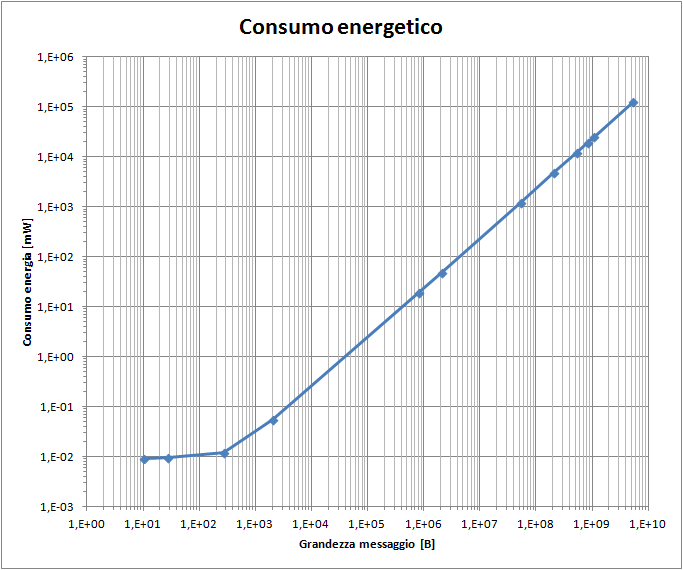
\includegraphics[width=0.8\linewidth]{Images/studio_energetico/cons_en_sing_tx_02}
	\caption[Studio energetico]{Energia media richiesta per il trasferimento di una informazione.}
	\label{fig:cons_en_sing_tx_02}
\end{figure}
Ovviamente i risultati ottenuti sia in termini di numero di trasmissioni possibili sia in termini di durata del dispositivo sono delle stime. Come già detto, il nostro modello lavora nell'ipotesi di maggior consumo energetico per vedere il comportamento nel suo caso pessimo. Anche per grandezza dell'informazione abbiamo voluto vedere anche qualche caso limite come quelli da $1\,GB$ e da $5\,GB$. Vi riportiamo i risultati nei grafici in \myFig{fig:numero_trasmissioni} e \myFig{fig:durata}. Dai risultati ottenuti si nota come per informazioni fino a $2\,KB$ non sia nessuna differenza sia in termini di numero di trasmissioni possibili sia di autonomia. I valori ottenuti rimangono "accettabili" fino a $200\,MB$, per poi subire un forte degrado per i valori più grandi, da $500\,MB$ a $5\,GB$.

Lo studio energetico ci ha confermato che il BLE è una tecnologia in grado di soddisfare le nostre necessità e, come esporremo nel capitolo successivo, è stata scelta per lo sviluppo della soluzione. Ora che abbiamo capito quale fosse il nostro punto di partenza, abbiamo impostato il problema di ricerca, dedicandoci allo studio di un modello di rete che potesse descrivere correttamente la disposizione dei dispositivi, del mezzo di comunicazione e del sistema di regole che governa la diffusione delle informazioni

\begin{figure}[t]
	\centering
	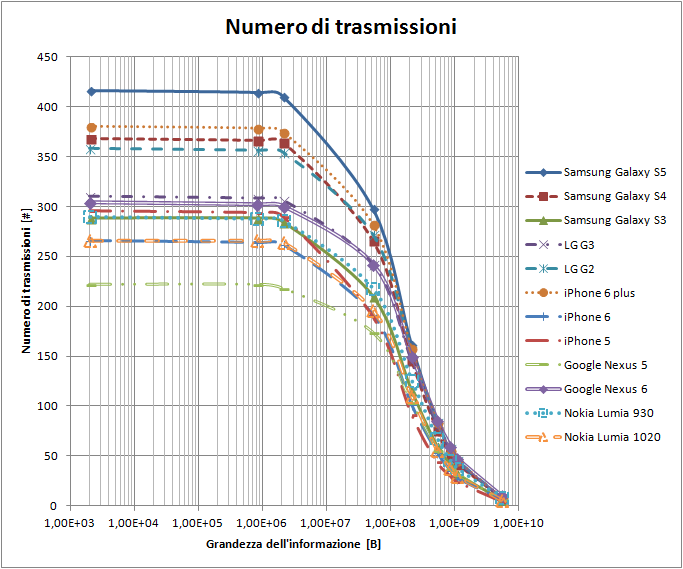
\includegraphics[width=0.8\textwidth, keepaspectratio]{Images/studio_energetico/numero_trasmissioni}
	\caption[Numero di trasmissioni.]{Numero di trasmissioni possibili.}
	\label{fig:numero_trasmissioni}
\end{figure}
\begin{figure}[t]
	\centering
	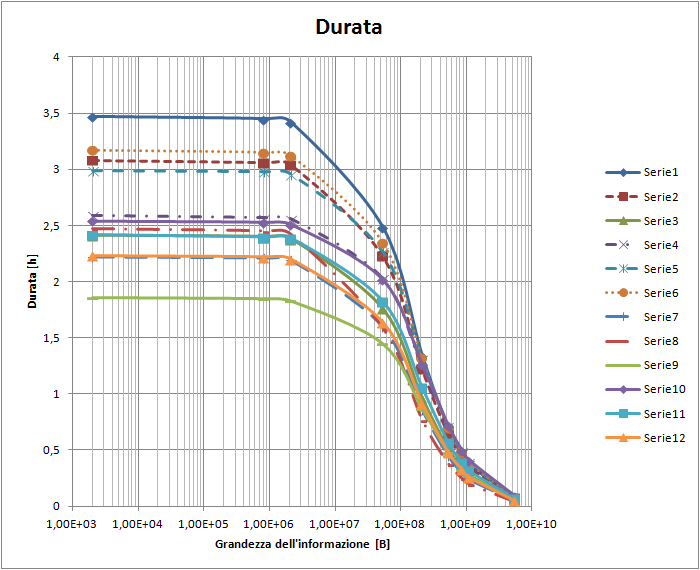
\includegraphics[width=0.8\textwidth, keepaspectratio]{Images/studio_energetico/durata}
	\caption[Durata]{Durata dei dispositivi.}
	\label{fig:durata}
\end{figure}